\section*{Analytic Geometry}
In this chapter we will add some geometric interpretation and intuition to all of these concepts. In particular, we will look at geometric vectors and comput their lengths and distances or angle between two vectors. To be able to do this, we equip the vector space with an inner product that induces the geometry of the vector space.
\begin{figure}[htbp]
    \centering
    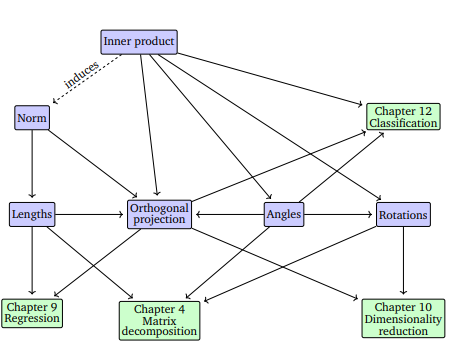
\includegraphics[width=11cm]{Analytical Geometry/mindmap.png}
\end{figure}
\subsection*{Norms}
\begin{definition}[Norm]
    A norm on a vector space V is a function 
    \begin{align*}
        \norm{\cdot}: &V \longrightarrow \mathbb{R}
        &x \mapsto \norm{x}
    \end{align*}
    which assigns each vector x its length $\norm{x} \in \mathbb{R}$, such that for all $\lambda \in \mathbb{R}$ and $x,y \in V$ the following hold: 
    \begin{itemize}
        \item Absolutely homogeneous: $\norm{\lambda x} = \absolute{\lambda}\norm{x}$
        \item Triangle inequality: $\norm{x+y} \leq \norm{x} + \norm{y}$
        \item Positive definite: $\norm{x} \geq 0$ an $\norm{x} = 0 \Longleftrightarrow x = 0$
    \end{itemize}
\end{definition}
The norm we will be using throughout these notes is going to be the Euclidean norm by default if not stated otherwise.
\begin{definition}[Euclidean Norm]
    The Euclidean norm of $x\in \mathbb{R}^n$ is defined as:
    \[ 
        \eunorm{x} = \sqrt[2]{\sum_{i=1}^{n}{x^2} = \sqrt{x^Tx}}
    \]and it computes the Euclidean distance from x to the origin. The Euclidean norm is also called the $\ell_2$ norm.
\end{definition}
\subsection*{Inner Products}
Recall the linear mappings where we can rearrange the mapping with respect to addition and multiplication with a scalar. A bilinear mapping $\Omega$ is a mapping with two arguments, and it is linear in each argument, i.e., when we look at a vector space V then it holds that for all $x,y,z \in V, \lambda, \psi \in \mathbb{R}$ that
\begin{align*}
    \Omega(\lambda x+ \psi y, z) = \lambda\Omega(x,y) + \psi\Omega(y,z)\\
    \Omega(x,\lambda y+ \psi z) = \lambda\Omega(x,y) + \psi \Omega(x,z)
\end{align*}
A bilinear mappings doesnt work on a single vector space but on the cartesian product of two vector spaces. We want to focus on biliear mappings that are: \begin{itemize}
    \item Symmetric: $\Omega(x,y)= \omega(y,x), \quad \forall x,y \in V$
    \item Positive definite: \[ 
        \forall x \in V\setminus\{0\} : \Omega(x,x) >0, \quad \Omega(\vec{0},\vec{0})= 0
    \]
\end{itemize}
\begin{definition}[Inner product]
    Let V be a vector space and $\Omega: V \times V \longrightarrow \mathbb{R}$ be a bilinear mapping that takes two vectors and maps them onto a real number. Then
    \begin{itemize}
        \item A positive definite, symmetric bilinear mapping $\Omega: V \times V \longrightarrow \mathbb{R}$ is called an inner product on V. We typically write $\anglepar{x,y}$ instead of $\Omega(x,y)$.
        \item The pair $(V,\anglepar{\cdot, \cdot})$ is called an inner product space or (real) vector space with inner product. If we use the dot product we call $(V,\anglepar{\cdot, \cdot})$ a Euclidean vector space. We will refer to these spaces as inner product spaces. 
    \end{itemize}
\end{definition}
Recall that any vectors $x,y \in V$ can be written as linear combinations of the basis vectors so that $x = \sum_{i=1}^{n}{\psi_i b_i} \in V$ and $y = \sum_{j=1}^{n}{\lambda_j b_j} \in V$ for suitable $\psi_i,\lambda_j \in \mathbb{R}$. Due to the bilinearity of the inner product, it holds for all $x,y \in V$ that
\[ 
    \anglepar{x,y} = \anglepar{\sum_{i=1}^{n}{\psi_ib_i}, \sum_{j=1}^{n}{\lambda_j b_j}} = \sum_{i=1}^{n}{\sum_{j=1}^{n}{\psi_i\anglepar{b_i,b_j}\lambda_j}} = \hat{x}A\hat{y}
\]where $A_{i,j} := \anglepar{b_i,b_j}$ and $\hat{x},\hat{y}$ are the coordinates of x and y with respect to the basis B. This implies that the inner product $\anglepar{\cdot, \cdot}$ is uniquely determined through A. The symmetry of the inner product also means that A is symmetric. Furthermore, the positive definiteness of the inner product implies that
\[ 
    \forall x \in V \setminus\{0\} : x^TAx>0
\]
\begin{definition}[Symmetric, Positive Definite Matrix]
    A symmetric matrix $A \in \mathbb{R}^{n\times n}$ that satisfies 
    \[ 
        \forall x \in V \setminus\{0\} : x^TAx>0 
    \]
    is called symmetric, positive definite or just positive definite. 
\end{definition}

\subsection*{Lengths and Distances}
\begin{remark}[Cauchy-Schwarz inequality]
    For an inner product vector space $(V, \anglepar{\cdot, \cdot})$ the induced norm $\norm{\cdot}$ satisfies the Cauchy-Schwarz inequality 
    \[ 
        \absolute{\anglepar{x,y}} \leq \norm{x}\norm{y} 
    \]
\end{remark}
\begin{definition}[Distance and Metric]
    Consider an inner product space $(V, \anglepar{\cdot, \cdot})$. Then 
    \[ 
        d(x,y):= \norm{x-y} = \sqrt{\anglepar{x-y,x-y}}
    \]is called the distance between x and y for $x,y \in V$. If we use the dot product as the inner product, then the distance is called Euclidean distance.\\
    The mapping
    \begin{align*}
        d: &V \times V \longrightarrow \mathbb{R}\\
        &(x,y) \mapsto d(x,y)
    \end{align*}
\end{definition}
A metric $d$ satisfies the following:
\begin{itemize}
    \item $d$ is positive definite, i.e., $d(x,y) \geq 0\; \forall x,y \in V$ and $d(x,y) = 0 \Longleftrightarrow x=y$
    \item $d$ is symmetric, i.e., $d(x,y) = d(x,y)\; \forall x,y \in V$
    \item Triangle inequality: $d(x,z) \leq d(x,y)+d(y,z) \; \forall x,y,z \in V$
\end{itemize}
\begin{remark}
    At first glance, the lists of properties of inner products and metrics look very similar. However, we observe that $\anglepar{x,y}$ and $d(x,y) $ behave in opposite directions. Very similar x and y will result in a large value for the inner product and a small value for the metric.
\end{remark}
\subsection*{Angles and Orthogonality}
In addition to enabling the definition of lenghts of vectors, as well as the distance between two vectors, inner products also capture the geometry of a vector space by defining the angle $\omega$ between two vectors. We use the Cauchy-Schwarz inequality to define angles $\omega$ in inner product spaces between two vectors x,y, and this notation coincides with our intuition in $\mathbb{R}^2$ and $\mathbb{R}^3$. Assume that $x \neq 0, y\neq 0$. Then 
\[ 
    -1 \leq \frac{\anglepar{x,y}}{\norm{x}\norm{y}} \leq 1 
\]
Therefore, there exists a unique $\omega \in [0,\pi]$ with 
\[ 
    \cos{\omega} = \frac{\anglepar{x,y}}{\norm{x}\norm{y}}
\]Intuitively, the angle between two vectors tells us how similar their orientations are.
\begin{definition}[Orthogonality]
    Two vectors $x$ and $y$ are orthogonal if and only if $\anglepar{x,y} = 0$ and we write $x \perp y$. If additionally $\norm{x} = 1 = \norm{y}$, the vectors x and y are orthonormal.
\end{definition}
\begin{definition}[Orthogonal Matrix]
    A square matrix $A \in \mathbb{R}^{n\times n}$ is an orthogonal matrix if and only if its columns are orthonormal so that 
    \[ 
        AA^T = I = A^TA 
    \]which implies that
    \[ 
        A^{-1} = A^T 
    \]
\end{definition}
\subsection*{Orthonormal Basis}
\begin{definition}[Orthonormal Basis]
    Consider an n-dimensional vector space V and a basis $b_{1}, \ldots,b_{n}$ of V. If 
    \begin{align*}
        \anglepar{b_i,b_j} = 0 \; for \; i\neq j \\
        \anglepar{b_i,b_j} = 1
    \end{align*}
    for all $i,j = 1, \ldots, n$ then the basis is called an orthonormal basis (ONB).
\end{definition}